\chapter{Introduction}
\section{Micro-Controllers and their specifications}
\subsection{Raspberry Pi 3B}
\par  Raspberry Pi (RPi) is an on-board computer and it is among the most popular development boards. The Raspberry Pi runs a customized version of Linux called Raspberry Pi OS. It has all the features of a personal computer. This board has USB interfaces that allow it to connect to peripherals (such as a mouse and keyboard), USB storage, etc. HDMI interface can be used to connect displays to the board having up to 4K resolution. Additionally, it has other ports/interfaces, including USB-C (power), a 2-lane MIPI CSI port (camera), a 3.5mm audio jack (audio), and RJ-45 (Ethernet). WiFi and Bluetooth 5.0 support are provided by the Raspberry Pi.

\begin{figure}[h!]
\centering
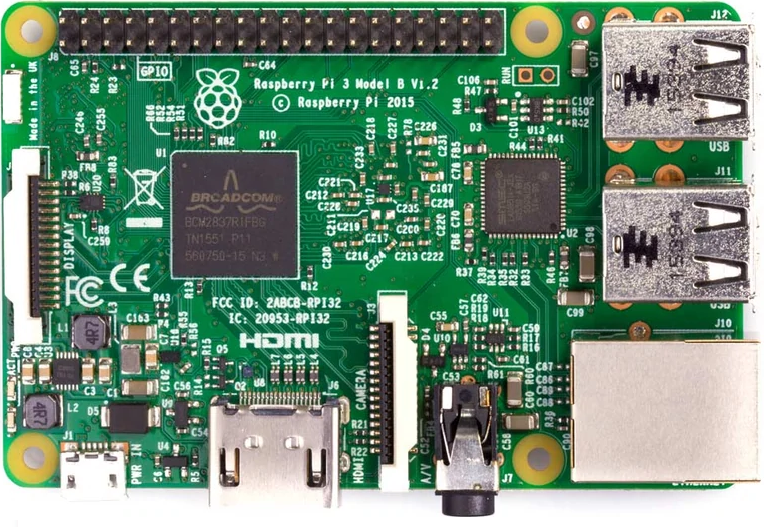
\includegraphics[width=9cm]{./Figures/Rpi_3B.png}
\caption{Raspberry Pi 3B}
\label{Rpi_3B}
\end{figure}

\subsection{ESP32} 
\begin{figure}[h!]
\centering
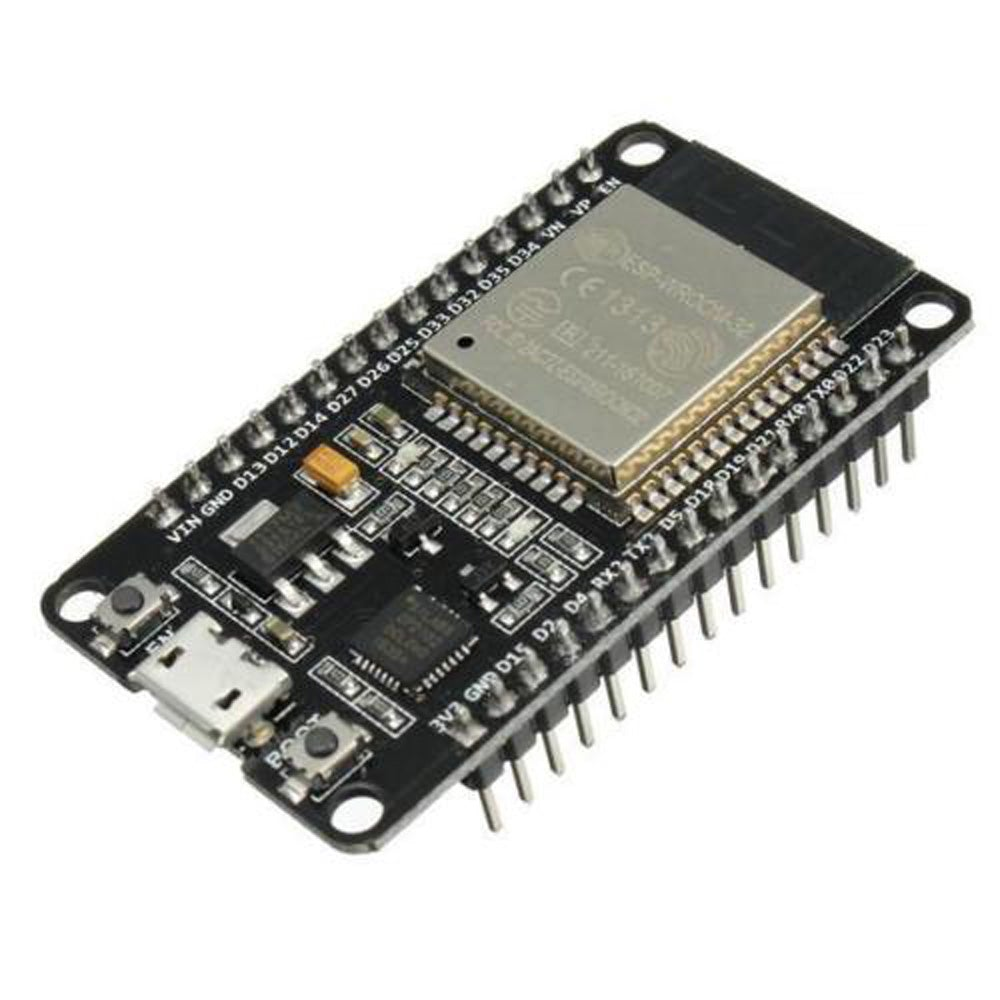
\includegraphics[width=5cm]{./Figures/ESP32.jpg}
\caption{ESP-WROOM-32 Dev Kit}
\label{ESP32}
\end{figure}
\par  ESP32 is a family of low cost and low power system on a chip (SoC) micro-controllers. It is enabled with dual mode bluetooth and integrated Wi-Fi.It is a successor to the ESP8266 micro-controller. Tensilica Xtensa 32-bit LX6 is main processor inside ESP32. It has memory of 320 KiB RAM and 448 KiB ROM. It contains 34 programmable GPOIs, 12-bit SAR ADC up to 18 channels, two 8-bit DACs, four SPI, two I2S and I2C and three UART interfaces.I have used ESP32-WROOM-32 module for my projects.



\begin{longtable}{|l|c|c|c|}
%\centering

%\begin{tabular}{|l|c|c|c|}
\hline
\textbf{Parameters} & \textbf{Raspberry Pi 3B} & \textbf{ESP-32} \\ \hline
\textbf{Processor} & \begin{tabular}[c]{@{}c@{}}Quad-core Broadcom \\ BCM2837 (4×Cortex-A53)\end{tabular} & \begin{tabular}[c]{@{}c@{}}Xtensa Dual-Core 32-bit \\ LX6 with 600 DMIPS\end{tabular} \\ \hline
\textbf{GPU} & \begin{tabular}[c]{@{}c@{}}Broadcom VideoCore IV \\ @ 250 MHz\end{tabular} & - \\ \hline
\textbf{Operating voltage} & 5V & 3.3V \\ \hline
\textbf{Clock speed} & 1.2GHz & 26 MHz – 52 MHz \\ \hline
\textbf{System memory} & 1 GB & \textless{}45kB \\ \hline
\textbf{Flash memory} & - & up to 128MB \\ \hline
\textbf{EEPROM}  & - & - \\ \hline
\textbf{\begin{tabular}[c]{@{}l@{}}Communication \\ supported\end{tabular}} & \begin{tabular}[c]{@{}c@{}}IEEE 802.11 b/g/n\\ Bluetooth, Ethernet Serial\end{tabular} & IEEE 802.11 b/g/n \\ \hline
\textbf{\begin{tabular}[c]{@{}l@{}}Development \\ environments\end{tabular}} & \begin{tabular}[c]{@{}c@{}}Any linux \\ compatible IDE\end{tabular} & Arduino IDE, Lua Loader \\ \hline
\textbf{\begin{tabular}[c]{@{}l@{}}Programming \\ language\end{tabular}} & \begin{tabular}[c]{@{}c@{}}Python, C, C++, Java,\\ Scratch, Ruby\end{tabular} & Embedded C, C++ \\ \hline
\textbf{I/O Connectivity} & \begin{tabular}[c]{@{}c@{}}SPI DSI UART \\ SDIOCSI GPIO\end{tabular} & UART, GPIO \\ \hline
%\end{tabular}
\caption{Comparison between Raspberry Pi 3B and ESP-32}
\end{longtable}
